\documentclass[conference]{IEEEtran}
\usepackage[utf8]{inputenc}
\usepackage[T1]{fontenc}
\usepackage{amsmath}
\usepackage{amssymb}
\usepackage{graphicx}
\usepackage{booktabs}
\usepackage{tabularx}
\usepackage{enumitem}
\usepackage{hyperref}

\begin{document}

\title{Why Network Intrusion Detectors Fail Across Years:\\
Decomposing Cross-Year Failure into Covariate Shift, Concept Change,
and Prior-Probability Shift}

\author{\IEEEauthorblockN{Adrin Paudel}
\IEEEauthorblockA{Kathmandu, Nepal\\
adrin.bct78015@kecktm.edu.np, paudeladrin@gmail.com}}

\maketitle
\begin{abstract}
Machine-learning intrusion detectors score almost perfectly on the data they were trained on, then fail on traffic from a different year or network. Knowing that they fail does not fix them; a practitioner needs to know which part of the signal changed. We decomposed the cross-year failure of a tree-ensemble NIDS (LightGBM in random-forest mode) on the corrected CIC-IDS 2017 and 2018 datasets into three independent mechanisms: covariate shift (feature values move), concept change (a feature stops separating attack from benign), and prior-probability shift (the benign-to-attack balance changes). Two intuitive mitigations both failed. The belief that a model relies most on the features that drift most held only for biased native importance and vanished under unbiased permutation importance, which makes native importance a poor drift proxy. Selecting the most concept-stable features did not beat ordinary importance ranking in a retraining ablation. The benign-rate shift was a separate failure that feature selection could not touch, so we tested the recalibration it calls for: re-thresholding the trained model to the target-year prior lifted cross-year attack F1 from near zero to 0.64 where prior shift dominated, though covariate-shift collapse stayed near zero. Because the two years differ in testbed and infrastructure as well as capture date, part of the measured shift reads as cross-testbed generalization failure rather than drift on a fixed population. We report the decomposition, the negative results, and the one fix that worked, and we point the remaining effort toward threshold and prior recalibration rather than feature engineering alone.
\end{abstract}

\begin{IEEEkeywords}
network intrusion detection, temporal drift, covariate shift, concept drift, prior-probability shift, cross-year generalization, feature importance, LightGBM, CIC-IDS
\end{IEEEkeywords}

\section{Introduction}

A machine-learning network intrusion detection system (NIDS) usually reports near-perfect F1 when its test data comes from the same capture it was trained on, then detects almost nothing on traffic from a different year or network. Sommer and Paxson [1] named this laboratory-versus-deployment gap one of the most consequential open problems in applied network security, since a detector is only useful on traffic it has never seen.
\par\medskip

The usual explanation, that the model overfits to transient network artifacts, is true but not actionable. It does not say how much of the signal changed, which features drove the failure, or whether any principled fix closes the gap. Building a NIDS that generalizes requires knowing how it fails, because different features fail in different ways and each needs a different correction. Some features keep their meaning but shift in absolute value; some stop separating attack traffic from benign traffic; and, independent of any single feature, the benign-to-attack mix can change and miscalibrate the whole detector. We took the failure apart along these three lines.
\par\medskip

The question came from an observation during development. A detector trained on the standard CIC-IDS data was deployed in a controlled two-virtual-machine testbed: one VM ran normal user activity (web browsing) alongside the detector, the other played the attacker, and both were isolated from the Internet and connected only to each other. When the attack began, the detector's accuracy fell sharply, far below its laboratory scores.* To study the mechanism rigorously we turned to a controlled cross-year comparison on the corrected CIC-IDS 2017 and 2018 datasets, where both years were re-extracted by the same corrected tool so that measured differences reflected genuine temporal change, not tooling.
\par\medskip

\footnotesize * The two-virtual-machine deployment observation is the author's own motivating experiment, reported as a concrete, firsthand instance of the documented laboratory-to-deployment gap [1] rather than as a new claim; it is motivation only, not a measured result in this study.\normalsize\par\medskip

We studied a tree-ensemble NIDS (LightGBM in random-forest mode) on network-flow features, 81 extracted per flow and reduced to 71 by correlation-based redundancy removal (Section III-B). Two tasks were run: binary (benign vs. attack), which carried the full drift decomposition, both hypothesis tests, and the ablation; and multiclass (seven attack families), evaluated for cross-year transfer only (Section V-A) and not carried through the hypothesis tests. We split cross-year drift into two orthogonal per-feature axes, covariate shift and concept stability, and treated prior-probability shift as a third, independent mechanism. Two hypotheses framed the analysis, each tested across both axes. H1: as importance rises, features grow less stable on either axis, showing more value shift (Axis 1) and less concept stability (Axis 2). H2: selecting features by either stability axis improves cross-year transfer over importance-based selection. Both were negative under a conjunctive bar chosen to be hard to pass by chance (Section VI-D), and we report the negative findings as substantive results rather than a failed search for a positive one.
\par\medskip

\noindent\textbf{Contributions.}\par\smallskip

\begin{enumerate}[leftmargin=*,itemsep=2pt,topsep=2pt]
  \item A reusable per-feature decomposition that separates three ways cross-year traffic changes: raw value shift (covariate), loss of attack-vs-benign separability (concept), and prior-probability shift, each with a per-feature null floor.
  \item An honest two-axis test of the intuition that a model leans on the features that drift most. The intuition failed once concept stability was included: important features were, if anything, more concept-stable, not less, strongly so under native importance and never significantly the reverse under permutation importance. Native importance should therefore not serve as a drift-risk proxy on either axis.
  \item A retraining ablation, run against both stability axes, showing that selecting by axis1\_\allowbreak{}stable or axis2\_\allowbreak{}stable did not reliably beat ordinary importance ranking, a negative result that redirects mitigation effort.
  \item Identification of prior-probability shift as a separate, selection-proof failure, with a per-family ranking of which attacks transferred (BruteForce worst among families with an adequate 2017 sample; WebAttack best but on a small 2017 sample; see Section V-F and the Limitations). We then tested the recalibration this diagnosis implies and found it recovered most of the prior-shift-driven loss (Section VII).
\end{enumerate}

\section{Related Work}

\subsection{CIC-IDS Datasets and the Corrected Re-Extraction}

CIC-IDS 2017 [2] and CSE-CIC-IDS 2018 [3] (hereafter CIC-IDS 2018 for brevity) are, by a wide margin, the most widely used and most available labeled NIDS benchmarks with realistic background traffic and scripted attacks. While researching how to use them defensibly, we found a 2022 paper [5] reporting that the original CICFlowMeter extraction for both years (the tool Engelen et al. [4] had already shown contains systematic errors) was re-run on the same underlying packet captures with a corrected, fixed version of the tool, with the attacks relabeled. One difference from the original CIC release is a third label category, "Attempted," alongside "Benign" and the specific attack families: each attack type is split into its successful and attempted variants instead of folding both into one label. We used this corrected release for both years so that any measured drift reflects genuine network, attacker, or environmental change rather than extraction artifacts; the same pipeline would apply unchanged to other corrected benchmarks, but datasets produced by different extraction tools cannot be mixed into one cross-year study without reintroducing tool-level confounds.
\par\medskip

\subsection{Dataset Shift and Temporal Generalization}

Quiñonero-Candela et al. [6] formalized dataset shift, separating covariate shift (P(X) changes while P(Y|X) is stable) from concept drift (P(Y|X) changes), and Gama et al. [7] surveyed concept-drift adaptation. We named our per-feature measure of the latter concept stability (Section IV-C), to stress that we scored how well discrimination was preserved rather than how much it changed. In security, Pendlebury et al. [8] showed cross-time degradation for malware classifiers and argued for separating feature-distribution shift from decision-boundary shift, the distinction our covariate-vs-concept framings make operational. Recent NIDS work [9] documented similar degradation but usually attributed it to evolving attacks without decomposing the mechanism. Closest to our setting, Cantone et al. [15] reported near-chance cross-dataset accuracy for several ML-based NIDS across benchmark pairs in this same dataset family, establishing that the failure occurs; we took the complementary step of decomposing why, into separable covariate-shift, concept-stability, and prior-shift mechanisms. A concurrent study [16] evaluated temporal and enterprise-to-IoT transfer across datasets spanning 2017--2024 and reported comparable degradation, analyzing stability over semantically grouped feature categories; our per-feature, two-axis decomposition and retraining ablation work at finer granularity and test, rather than assume, whether importance or stability predicts transfer. A 2024 survey [17] noted that work connecting drift to specific features is scarce and proposed dynamic, drift-aware feature selection as a general mitigation; the ablation in Section VI-B tests that proposal directly for a tree-ensemble NIDS.
\par\medskip

\subsection{Feature Importance in Tree Ensembles}

Breiman [10] introduced permutation importance as an unbiased estimator; Strobl et al. [11] showed that native impurity-based importance measures, including the total-gain measure used as our native importance and the split-count variant recorded as a secondary diagnostic (Section IV-A), are biased toward high-cardinality features. That bias is central to interpreting H1, since both native importance and our covariate-shift metric tend to rise with feature cardinality and continuity.
\par\medskip

\section{Datasets and Preprocessing}

\subsection{Datasets}

We used the corrected CIC-IDS 2017 and 2018 datasets [5] as the two comparison points, rather than training on one and generating a second test set by replaying attacks against a live virtual-machine testbed, the design that first motivated this study (Section I) and that proved inconsistent run-to-run. Both years are independent captures of realistic traffic and attacks, so comparing them directly avoided the noise of simulated replay while preserving a genuine temporal gap, and both came from the same fixed extraction tool, so the measured shift reflected temporal difference rather than tooling. Table 1 summarizes the datasets after cleaning. The benign-to-attack balance differed sharply between the years, which became a result in its own right (Section V-E).
\par\medskip

\begin{table}[t]
\centering
\caption{Dataset Statistics After Cleaning}
\label{tab:1}
\footnotesize
\setlength{\tabcolsep}{3pt}
\begin{tabularx}{\columnwidth}{>{\raggedright\arraybackslash}p{0.48\columnwidth}>{\centering\arraybackslash}p{0.24\columnwidth}>{\centering\arraybackslash}X}
\toprule
\textbf{Property} & \textbf{CIC-IDS 2017} & \textbf{CIC-IDS 2018} \\
\midrule
Total rows (cleaned) & 2,099,960 & 63,195,088 \\
Train / test split (80/20) & 1,679,912 / 420,048 & 50,556,009 / 12,639,079 \\
P(benign), train split & 0.759 & 0.944 \\
P(attack), train split & 0.241 & 0.056 \\
|$\Delta$P(benign)| across years & 0.185 (LARGE) &  \\
Features retained & 71 & 71 \\
\bottomrule
\end{tabularx}
\end{table}

\subsection{Preprocessing Pipeline}

The raw extraction had 91 columns per flow. Of these, 9 were non-feature identifiers (source/destination IP and port, flow ID, row ID, protocol, timestamp, and the raw label) and 1, "Attempted Category," was consumed during cleaning to relabel attempted-but-unsuccessful attacks as Benign and then dropped, leaving 81 network-flow feature columns. Rows with NaN or infinite values were removed, along with exact duplicate rows, with row counts tracked at each stage; physically impossible values (e.g. negative packet lengths) were flagged during per-feature profiling but not dropped. Pearson and Spearman correlation matrices were computed per year; pairs flagged by both metrics in both years at r >= 0.95 were dropped by an mRMR minimum-redundancy rule (10 features dropped this way, e.g. Fwd Packet Length Mean and Fwd Segment Size Avg at r = 1.000 in both years), leaving 71 features (91 raw minus 9 identifiers, 1 "Attempted Category," and 10 redundant) in Table 1 for every downstream step, including training, testing, and the feature-selection ablation in Section IV-D. Features were then Z-score scaled, and two scaler artifacts were retained: the own-year scaler (for the concept framing) and the train-year scaler applied to target-year data (for the covariate framing). Attack labels were mapped to a common taxonomy of seven attack families plus Benign so both years share one label space.
\par\medskip

\section{Methodology}

\subsection{Model and Feature Importance}

Random-forest mode was chosen over LightGBM [12]'s default gradient-boosting mode for two reasons. First, in earlier unpublished iterations of this pipeline by the author, the model was scikit-learn's RandomForestClassifier, consistent with tree ensembles' established strength on network-flow tabular data [10], [11]; scaling to the corrected 2018 extraction's ~63M raw rows made scikit-learn's in-memory bootstrap-per-tree construction infeasible without capping the dominant Benign class, which would have distorted class-weight calibration. LightGBM's random-forest mode implements the same bagging-plus-feature-subsampling algorithm via histogram-based tree construction, preserving the trained model's RF semantics at full data scale instead of switching to a different ensembling algorithm for engineering convenience. Second, the paper's H1/H2 tests directly build on the native-vs-permutation importance bias analysis established for random forests [10], [11]; gradient-boosted trees compute importance over sequential residual fitting, a different semantics without the same bias characterization this study relies on. Each model used 200 trees, unrestricted depth, 255 leaves, per-tree row bagging fraction 0.632, per-split feature-subsample fraction 0.5, and class\_\allowbreak{}weight='balanced' (inverse-frequency reweighting against the training year's own class prior, applied identically to both years despite their differing benign/attack ratios); the full data was used without capping, and random\_\allowbreak{}state was fixed to seed 42 throughout. Training used LightGBM's GPU histogram, which is not bit-reproducible across hardware even at a fixed seed, so the reported numbers are from a single fixed-seed run rather than a bit-exact reproducible artifact. Feature importance was measured two ways: native (total split-gain, hereafter "gain"), which is fast but biased toward high-cardinality features [11] (split-count, a secondary diagnostic more biased still, was also recorded but not used for H1/H2); and permutation (balanced-accuracy drop when a feature is shuffled, 30 repeats), which is unbiased but noisier in the low-importance tail, a trade-off the repeat count bounds (Section VI-D). Reporting both mattered: they disagreed on whether Axis 1 alone was significant, though they agreed on the combined two-axis H1 verdict.
\par\medskip

\subsection{Cross-Year Evaluation Framings}

Each model was tested against the opposite year under two framings that isolate different failure mechanisms:
\par\medskip

\begin{itemize}[leftmargin=*,itemsep=2pt,topsep=2pt]
  \item Concept framing: target-year data scaled with its own year's scaler, which removed the raw value shift and isolated decision-boundary transfer.
  \item Covariate framing: target-year data scaled with the train-year scaler, which preserved the shift and simulated deployment, where no recalibration happens.
\end{itemize}

\subsection{The Two Drift Axes}

\textbf{Axis 1: Covariate shift.  }A Classifier Two-Sample Test (C2ST) [13] trains a classifier to distinguish a feature's 2017 values from its 2018 values: AUC near 0.5 means the distributions are indistinguishable, AUC near 1.0 means they are fully separable. A per-feature null floor from permuted year labels separates genuine shift from noise. Maximum Mean Discrepancy [14] and a shape-only Wasserstein distance serve as corroborating sub-metrics.\par\medskip

\textbf{Axis 2: Concept stability.  }Measures whether a feature still separates attack from benign in the later year, via a direction-aware product of its per-year separation strengths, scaled to [$-$1, +1]. Each year's strength is the larger of a folded separation-AUC and a normalized mutual-information score, so non-monotonic attack-vs-benign relationships are captured, not only monotone ones. Positive and large means the discrimination is preserved, near zero means it collapses, and negative means the attack-vs-benign relationship reverses sign (flipped).\par\medskip

\subsection{Hypotheses and the Decisive Ablation}

\textbf{H1.  }As feature importance rises, features become less stable on EITHER drift axis: more covariate shift (Axis 1, a positive correlation between importance and C2ST-AUC) and less concept stability (Axis 2, a negative correlation between importance and separation\_\allowbreak{}stability). Tested as 8 independent cells (native/permutation importance x 2017/2018 anchor year x Axis 1/Axis 2), each with its own Spearman rank correlation, cluster-robust (or plain) bootstrap 95\% CI, and Benjamini-Hochberg FDR correction across the 8-test family; H1 holds only if no cell contradicts it. The headline cells anchored importance to the training year (2017) to avoid circularity; the 2018-anchored cells were a robustness check.\par\medskip

\textbf{H2.  }Selecting features by EITHER stability axis, axis1\_\allowbreak{}stable (least value-drifted) or axis2\_\allowbreak{}stable (most concept-stable), yields better cross-year transfer than selecting by importance rank, in both transfer directions. Tested by a decisive cross-domain ablation: a fresh LightGBM model was retrained for each (K, policy) pair and evaluated in both transfer directions. Five policies were compared at K from 5 to 71: top\_\allowbreak{}importance, axis1\_\allowbreak{}stable, axis2\_\allowbreak{}stable, random, and all\_\allowbreak{}features (ceiling). Reported F1 values are relative policy comparisons on rebalanced test sets, not natural-prior deployment F1.\par\medskip

\section{Results}

\subsection{The Transfer Failure}

Within-year F1 was about 0.9997, but this is an inflated baseline, cited only to size the laboratory-versus-deployment gap, because near-identical flow records can straddle the train/test boundary. The real picture was the cross-year transfer in Table 2, which showed a marked asymmetry. The 2017 model transferred partially to 2018 under concept framing (attack F1 = 0.556) but almost not at all under covariate framing (attack F1 = 0.044), so most of the deployment loss in that direction was raw value shift, not decision-boundary collapse, and recalibrating the scaler recovered much of it. The 2018 model transferred poorly in the reverse direction, with the framings inverted: its concept-framing transfer collapsed entirely (attack F1 near 0) even though ranking quality held (ROC-AUC = 0.877). What failed was the implicit decision threshold, not the learned ranking, consistent with the prior-shift mechanism of Section V-E. Concept-framing recall was near zero (0.00005): the threshold learned on a 94\%-benign 2018 stream sat above nearly every 2017 attack score, so almost nothing was flagged despite good ranking. Under covariate framing the mismatched train-year scaler distorted the 2017 values just enough to push some attack scores back across that frozen threshold, lifting recall to 0.25 and attack F1 to 0.393, the opposite of the 2017-to-2018 pattern. That recovery was therefore a scaling mismatch partly compensating a miscalibrated threshold, not genuine feature transfer. This direction-dependent inversion is a structural asymmetry that feature handling alone cannot fix. Multiclass transfer was uniformly poor.
\par\medskip

\begin{table}[t]
\centering
\caption{Cross-Year Binary Transfer (All 71 Features)}
\label{tab:2}
\footnotesize
\setlength{\tabcolsep}{2pt}
\begin{tabularx}{\columnwidth}{>{\raggedright\arraybackslash}p{0.34\columnwidth}>{\centering\arraybackslash}p{0.145\columnwidth}>{\centering\arraybackslash}p{0.145\columnwidth}>{\centering\arraybackslash}p{0.145\columnwidth}>{\centering\arraybackslash}p{0.145\columnwidth}}
\toprule
\textbf{Direction / Framing} & \textbf{Macro F1} & \textbf{Attack F1} & \textbf{ROC-AUC} & \textbf{MCC} \\
\midrule
2017$\rightarrow$2018 concept & 0.756 & 0.556 & 0.934 & 0.567 \\
2017$\rightarrow$2018 covariate & 0.506 & 0.044 & 0.829 & 0.049 \\
2018$\rightarrow$2017 concept & 0.432 & 0.000 & 0.877 & 0.005 \\
2018$\rightarrow$2017 covariate & 0.642 & 0.393 & 0.919 & 0.433 \\
\bottomrule
\end{tabularx}
\end{table}

\footnotesize Table 2 reports point estimates on the full test set, without bootstrap confidence intervals (unlike the correlation results in Section V-C, which are interval-tested); the qualitative pattern (concept vs. covariate asymmetry, direction-dependent inversion) is large relative to plausible test-set sampling noise, but the exact digits should be read as point estimates, not interval-tested claims.\normalsize\par\medskip

\subsection{Decomposing the Drift: The Two Axes}

Across all 71 features, mean raw covariate shift (Axis 1, C2ST-AUC) was 0.666; calibrated against each feature's own permutation-null floor, the value used throughout, the mean was 0.309. The most shifted features were inter-arrival-time and flow-rate statistics (Fig. 1), quantities that track environment-level change between the two captures. Placing every feature on both axes (Figs. 2--3) gave four readable groups: features the model relied on that stayed discriminative, fragile shortcuts that were relied on but unstable, noise, and a reserve of stable but under-used features. Fig. 4 summarizes the per-feature drift verdicts (27 shifted, 23 restructured, 9 weak, 6 flipped, 3 collapsed, 3 stable); only 3 of 71 features were statistically indistinguishable across the two years.
\par\medskip

\begin{figure}[t]
\centering
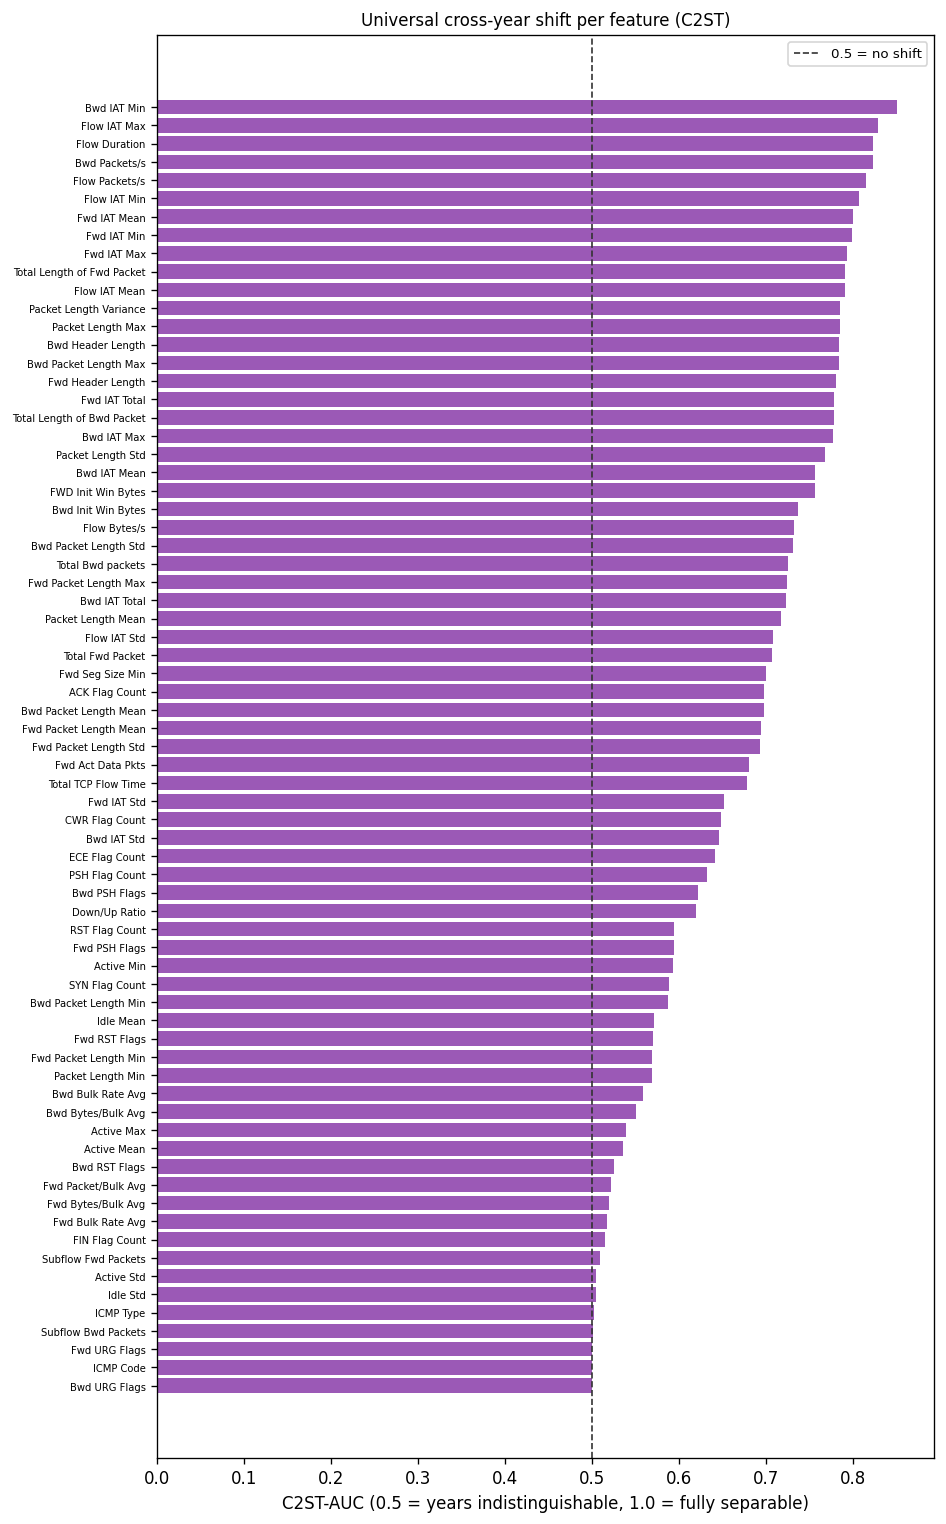
\includegraphics[width=\linewidth]{results/11_cross_analysis/lightgbm/c2st_bar.png}
\caption{Covariate shift (C2ST-AUC) for all 71 features, sorted. 0.5 = indistinguishable across years, 1.0 = fully separable. Inter-arrival-time and flow-rate features shift most.}
\label{fig:1}
\end{figure}

\begin{figure}[t]
\centering
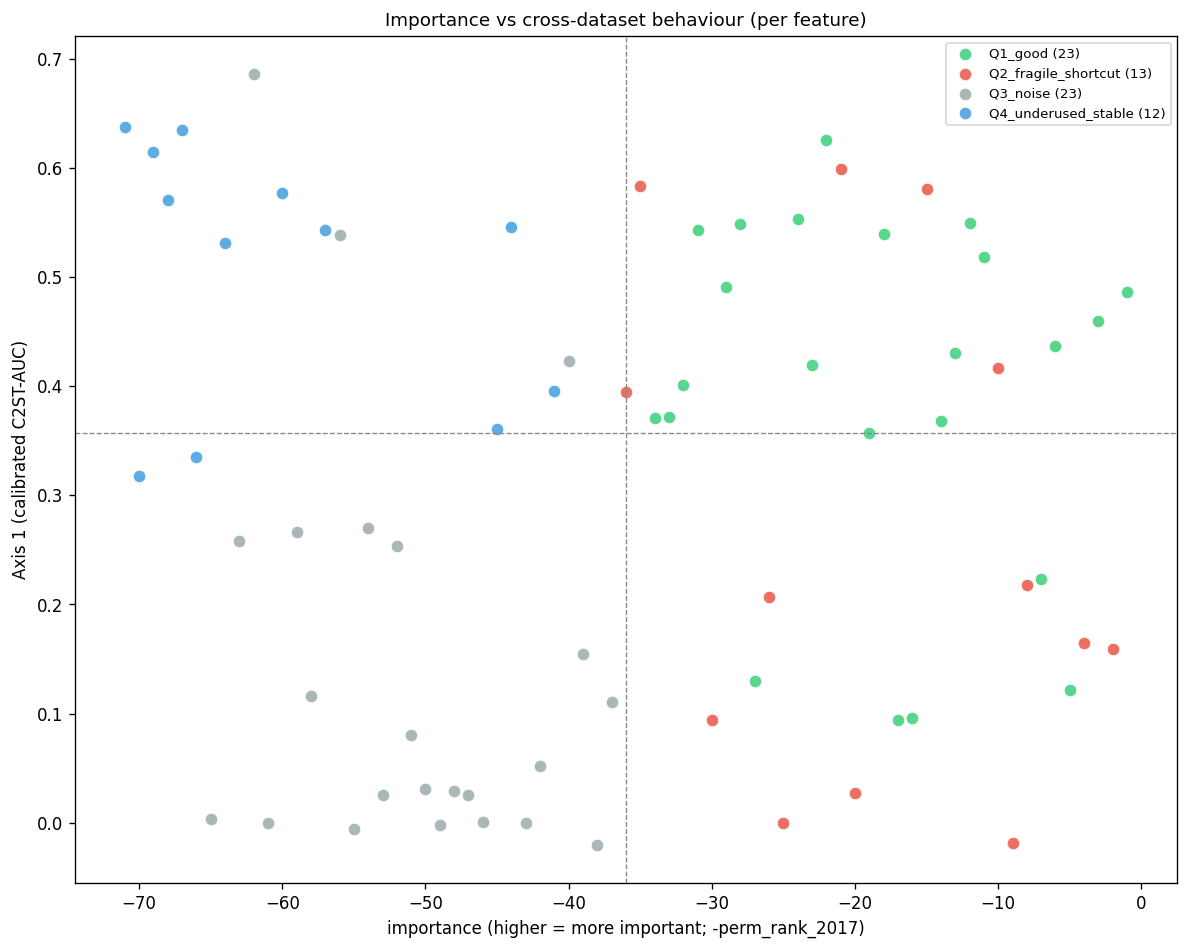
\includegraphics[width=\linewidth]{results/11_cross_analysis/lightgbm/quadrant_axis1.png}
\caption{Every feature placed by 2017 permutation importance (horizontal) and calibrated covariate shift, Axis 1 (vertical): the same quadrant view as Fig. 3, split out for the shift axis.}
\label{fig:2}
\end{figure}

\begin{figure}[t]
\centering
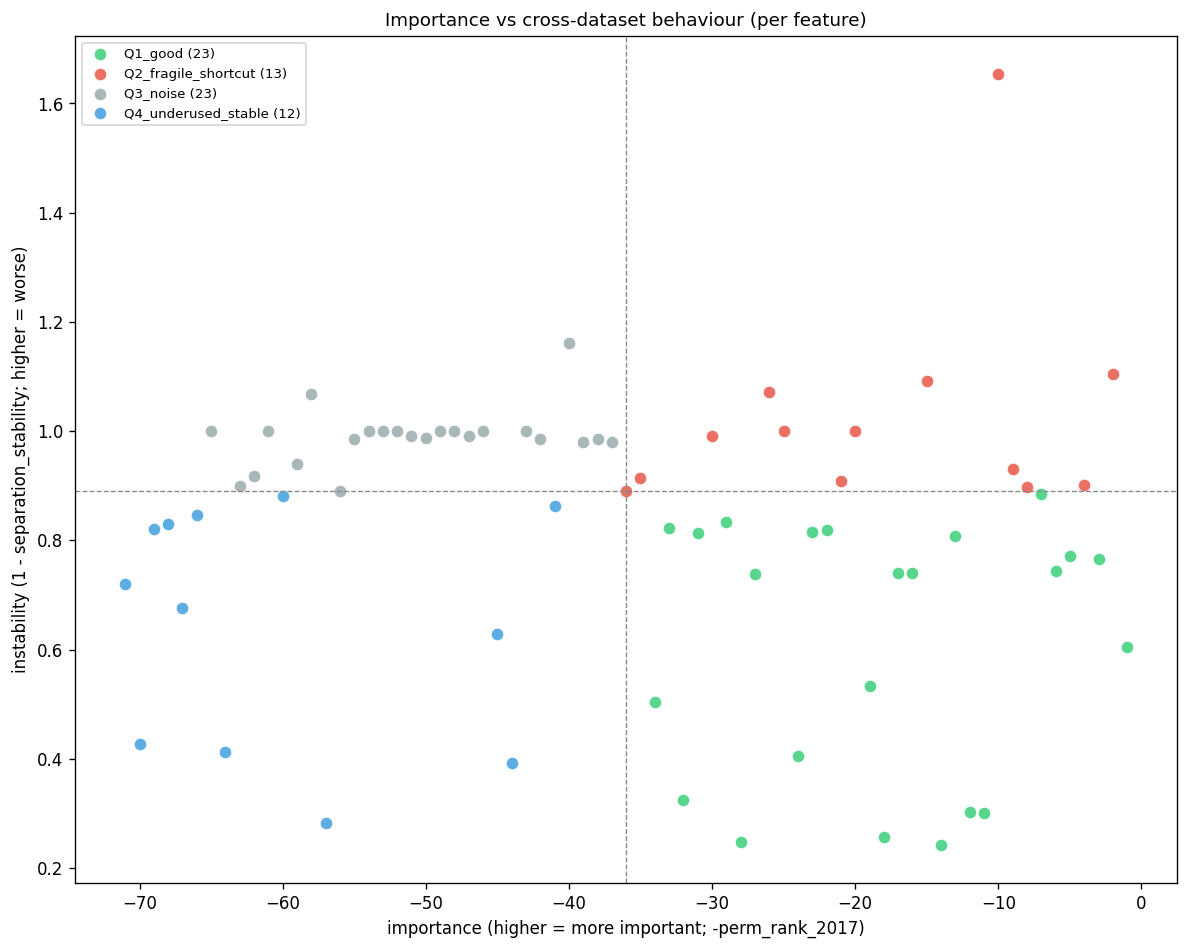
\includegraphics[width=\linewidth]{results/11_cross_analysis/lightgbm/quadrant_axis2.png}
\caption{Every feature placed by 2017 permutation importance (horizontal) and concept instability (1 $-$ separation stability), Axis 2 (vertical): relied-on-and-stable, fragile shortcuts, noise, and an under-used stable reserve.}
\label{fig:3}
\end{figure}

\begin{figure}[t]
\centering
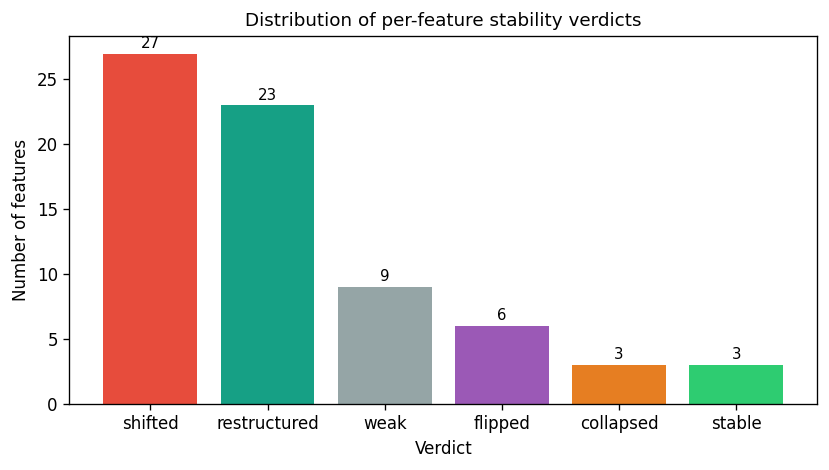
\includegraphics[width=\linewidth]{results/11_cross_analysis/lightgbm/verdict_distribution.png}
\caption{Distribution of per-feature drift verdicts (shifted, restructured, weak, flipped, collapsed, stable) from the two-axis analysis. Only 3 of 71 features are stable across years.}
\label{fig:4}
\end{figure}

\subsection{H1: Importance vs. Both Drift Axes}

The intuition that a model leans hardest on the features that move most, and only those, is at best half the picture once both drift axes are checked across all 8 importance-variant x axis cells, and is contradicted once the second axis is included. On Axis 1 (covariate shift), native importance correlated positively with C2ST-AUC under both anchor years (2017: $\rho$ = +0.41, 95\% CI [+0.16, +0.61], BH-FDR q = 0.008; 2018: $\rho$ = +0.59, CI [+0.37, +0.79], q < 0.001), both surviving FDR correction; under unbiased permutation importance (30 shuffles) this Axis-1 signal was weak and did not survive correction in either year (2017: $\rho$ = 0.00, CI [$-$0.24, +0.30], q = 0.95; 2018: $\rho$ = +0.20, CI [$-$0.08, +0.46], q = 0.20). On Axis 2 (concept stability), however, importance correlated POSITIVELY with separation\_\allowbreak{}stability under native importance in both years (2017: $\rho$ = +0.46, CI [+0.23, +0.66], q < 0.001; 2018: $\rho$ = +0.57, CI [+0.37, +0.72], q < 0.001) and under 2018 permutation importance ($\rho$ = +0.34, CI [+0.06, +0.58], q = 0.024), the opposite of the sign H1 requires; only the 2017 permutation cell was inconclusive ($\rho$ = +0.15, CI [$-$0.09, +0.37], q = 0.25). Overall, Axis 1 was confirmed (right sign, CI excluding zero) in 2 of the 4 importance variants, both native; Axis 2 was contradicted (wrong sign, CI excluding zero) in 3 of 4, and inconclusive, never supportive, in the fourth. Because H1 requires reduced stability on Axis 2, and no Axis-2 cell supported that prediction, H1 is contradicted rather than merely unsupported under one estimator. The native-importance Axis-1 correlation is itself partly an artifact of cardinality bias [11]: high-cardinality continuous features earn inflated native importance and also tend to show larger covariate shift, and correcting the estimator (permutation) removes that link, and with it most of the only axis on which H1 had any support. The class-mixture (prior) change in Section V-E contributed as well.
\par\medskip

\textbf{H1 verdict: }\textbf{\textit{contradicted. }}Native and permutation importance agreed: importance did not predict reduced stability on the concept axis, and if anything the opposite held. The apparent Axis-1-only support is therefore not evidence for H1 as stated. Importance does not generally mean "less stable."\par\medskip

\subsection{H2: The Decisive Ablation}

Retraining the real model on competing feature subsets (Fig. 5, Table 3) settled H2 directly, now with both stability axes head-to-head against importance-based selection rather than concept stability alone. The metric was Macro F1 (mean of Attack F1 and Benign F1), matching the H2 verdict itself rather than attack-class F1 alone. Per direction, top\_\allowbreak{}importance clearly led axis2\_\allowbreak{}stable in 2017-to-2018 (0.661 vs. 0.455); in 2018-to-2017 the two were nearly tied, with axis2\_\allowbreak{}stable edging top\_\allowbreak{}importance by a thin margin (0.512 vs. 0.501). axis1\_\allowbreak{}stable lost in both directions (0.258 vs. 0.661; 0.437 vs. 0.501) and was the worst of the five policies. H2 requires a stability policy to win in both directions, and neither did: axis2\_\allowbreak{}stable won at most one direction, by a margin too thin to call decisive, and axis1\_\allowbreak{}stable won neither. Averaged over K and both directions, top\_\allowbreak{}importance (mean cross-Macro-F1 0.581) led axis2\_\allowbreak{}stable (0.484), random (0.431), and axis1\_\allowbreak{}stable (0.348); that average is not the basis for the verdict, which rests on the stricter must-win-both-directions criterion above. In the 2017-to-2018 direction, importance-based selection showed a sharp onset between K = 10 and K = 20: a few individually top-ranked features were insufficient at K = 10 (Macro F1 = 0.383), but the joint structure was largely captured by K = 20 (Macro F1 = 0.859), a critical-mass effect rather than a smooth ramp. All-features gave the smallest generalization gap of any policy (0.279 vs. 0.414--0.566 for the four K-limited policies, Fig. 6).
\par\medskip

\begin{figure}[t]
\centering
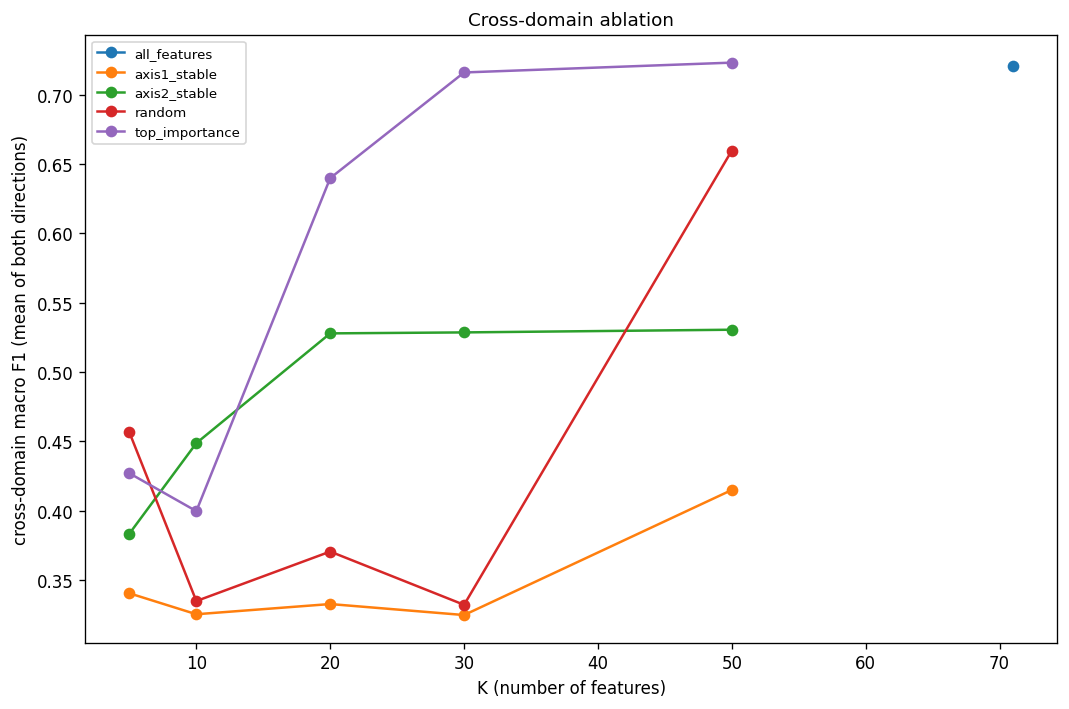
\includegraphics[width=\linewidth]{results/11_cross_analysis/lightgbm/ablation_crossdomain_f1.png}
\caption{Cross-domain Macro F1 (concept framing) vs. number of features K for each selection policy. Importance-based selection peaks highest in 2017$\rightarrow$2018; all policies drop sharply in 2018$\rightarrow$2017.}
\label{fig:5}
\end{figure}

\begin{figure}[t]
\centering
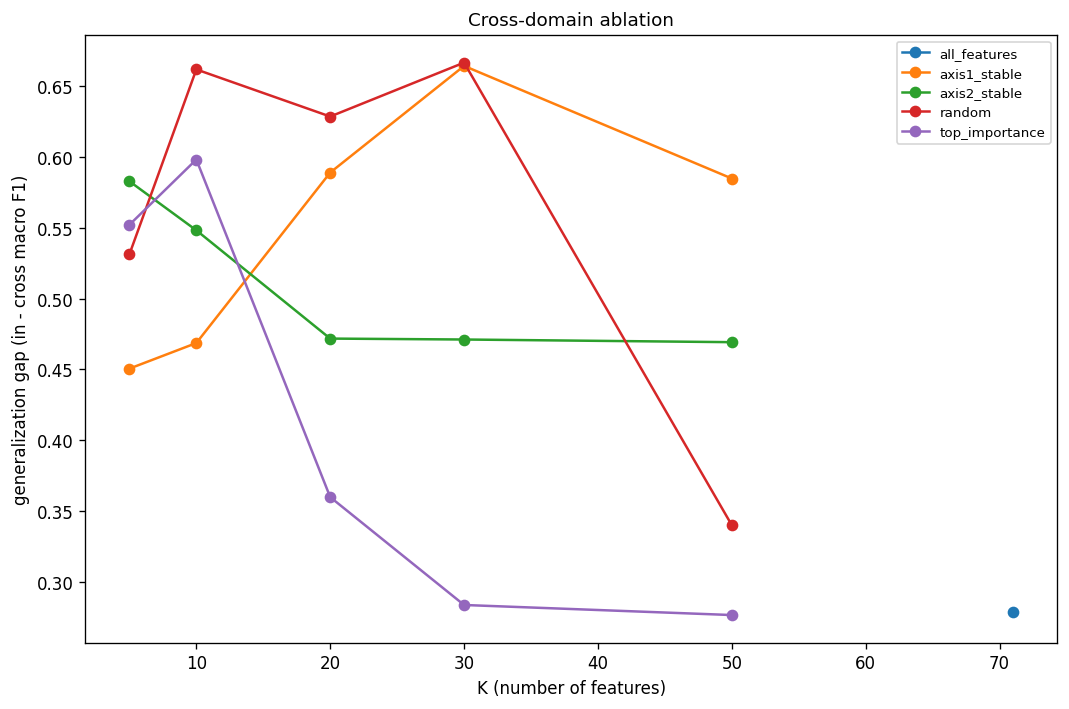
\includegraphics[width=\linewidth]{results/11_cross_analysis/lightgbm/ablation_gap.png}
\caption{Generalization gap (within-year F1 minus cross-domain F1) vs. K for each policy. all\_\allowbreak{}features has the smallest gap of any policy; the four K-limited policies all generalize worse.}
\label{fig:6}
\end{figure}

\begin{table}[t]
\centering
\caption{Cross-Domain Ablation Summary (Concept Framing, Macro F1, Averaged over K and Both Directions)}
\label{tab:3}
\footnotesize
\setlength{\tabcolsep}{3pt}
\begin{tabularx}{\columnwidth}{>{\raggedright\arraybackslash}p{0.27\columnwidth}>{\centering\arraybackslash}p{0.46\columnwidth}>{\centering\arraybackslash}X}
\toprule
\textbf{Policy} & \textbf{Mean Cross-Macro-F1 (Concept)} & \textbf{Mean Gen. Gap} \\
\midrule
all\_\allowbreak{}features & 0.721 & 0.279 \\
top\_\allowbreak{}importance & 0.581 & 0.414 \\
axis2\_\allowbreak{}stable & 0.484 & 0.509 \\
random & 0.431 & 0.566 \\
axis1\_\allowbreak{}stable & 0.348 & 0.551 \\
\bottomrule
\end{tabularx}
\end{table}

\textbf{H2 verdict: }\textbf{\textit{not supported on either axis. }}Neither axis1\_\allowbreak{}stable nor axis2\_\allowbreak{}stable clearly beat importance-based selection in both transfer directions, so feature selection by either stability criterion is not the lever that fixes cross-year transfer.\par\medskip

\subsection{Prior-Probability Shift: A Separate Failure}

Independent of any single feature, the benign rate rose from 75.9\% in 2017 to 94.4\% in 2018, a shift of |$\Delta$P| = 0.185 (Fig. 7). A model trained to expect roughly a quarter of traffic to be attacks is miscalibrated on a stream that is only 5.6\% attacks: its implicit decision threshold sits wrong and degrades precision regardless of how well individual features transfer. This is a direct instance of the base-rate fallacy, long known to dominate intrusion-detection performance [18]. Neither drift axis captures the mechanism, and feature selection cannot correct it, so we treated it as a first-class result and, in Section VII, tested the recalibration it calls for.
\par\medskip

\begin{figure}[t]
\centering
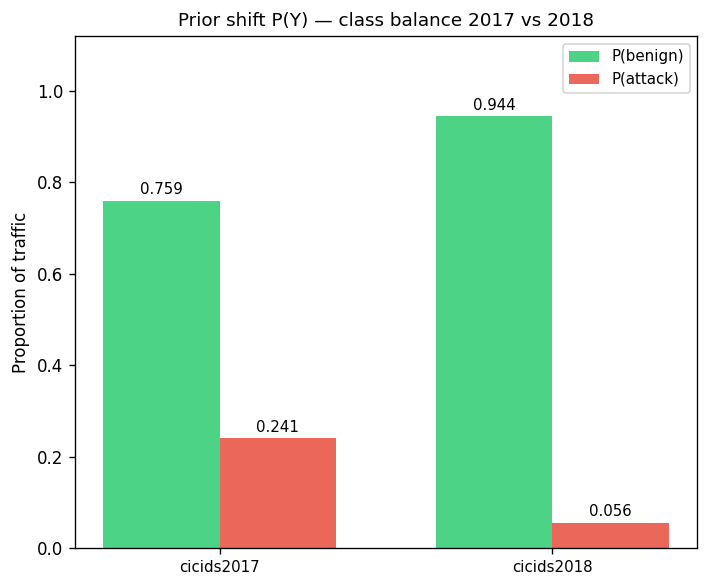
\includegraphics[width=\linewidth]{results/11_cross_analysis/lightgbm/prior_shift_bar.png}
\caption{Class-prior shift: P(benign) rises from 0.759 to 0.944 (|$\Delta$P| = 0.185). This independently degrades deployed precision and is not captured by either drift axis.}
\label{fig:7}
\end{figure}

\subsection{Which Attacks Transfer, and What Drives the Drift}

Attack families differed sharply in how well they transferred (Table 4), and the stability columns did not rank them the same way, so we name the metric behind each claim rather than treating "least stable" as a single score. By median separation stability and by the number of features whose attack-vs-benign relationship reversed sign ("\# Flipped"), BruteForce was the least stable family (18 flipped features, the most of any). The \% Stable column disagreed: DDoS and DoS were lower there (2.4\% vs. BruteForce's 15.7\%), so that column alone would not single out BruteForce. BruteForce's instability was partly a labeling artifact rather than pure attacker evolution. The attempted-to-Benign fold (Section III-B) removed every FTP-BruteForce flow from 2018 (each carried the "- Attempted" suffix), so the 2018 family was SSH-BruteForce only while the 2017 family combined FTP-Patator and SSH-Patator; the family's tool composition, not only the network, differed between years. Median covariate shift ranked the families differently again: Infiltration was the most stable by a wide margin (0.047), whereas WebAttack, despite keeping the most discriminative structure by separation stability, \% Stable, and \# Flipped, had the third-highest median shift (0.741, behind Botnet's 0.898 and DDoS's 0.758). A feature's attack-vs-benign relationship could stay intact (concept-stable) even as its raw values moved (covariate-shifted), which is why we measured and reported the two axes separately. PortScan does not appear in Table 4 because the corrected 2018 re-extraction contains no PortScan-labeled flows, leaving no stability axis to compute. Two further observations sharpened the picture. Attack-side distributions changed more than benign-side ones in 58 of 71 features (mean calibrated attack shift 0.558 vs. benign 0.323), pointing to adversary evolution over environment change. And a single-feature transfer test, using each feature alone as a threshold classifier and scoring whether its separation AUC stayed above a fixed cutoff in both years, found only 9 of 71 features transferred well on their own, with several high-importance features among the worst, confirming that cross-year signal lives in feature combinations, not individual columns.
\par\medskip

\begin{table}[t]
\centering
\caption{Attack-Family Stability, Sorted Least Stable First by Median Separation Stability (6 of 7 Families Shown; PortScan Excluded, See Text). The 2017 flows column is the family's total 2017 sample; WebAttack (104) and Botnet (736) are small, so their per-family stability ranks carry wide, unreported uncertainty (see Limitations)}
\label{tab:4}
\footnotesize
\begin{tabularx}{\columnwidth}{>{\raggedright\arraybackslash}X>{\centering\arraybackslash}X>{\centering\arraybackslash}X>{\centering\arraybackslash}X>{\centering\arraybackslash}X>{\centering\arraybackslash}X}
\toprule
\textbf{Family} & \textbf{2017 flows} & \textbf{Med. Sep. Stab.} & \textbf{Med. Shift (Calib.)} & \textbf{\% Stable} & \textbf{\# Flipped} \\
\midrule
BruteForce & 6,933 & 0.016 & 0.663 & 15.7\% & 18 \\
DDoS & 95,144 & 0.029 & 0.758 & 2.4\% & 8 \\
DoS & 171,634 & 0.036 & 0.647 & 2.4\% & 3 \\
Botnet & 736 & 0.039 & 0.898 & 6.0\% & 9 \\
Infiltration & 71,803 & 0.159 & 0.047 & 27.7\% & 2 \\
WebAttack & 104 & 0.258 & 0.741 & 31.3\% & 1 \\
\bottomrule
\end{tabularx}
\end{table}

\footnotesize Med. Sep. Stab. = median per-feature concept-stability score (Axis 2) within the family; Med. Shift (Calib.) = median per-feature covariate-shift calibrated C2ST-AUC (Axis 1); \% Stable = features with separation stability > 0.5; \# Flipped = features whose attack-vs-benign relationship reverses sign. Family statistics were computed over 83 features, a broader set than the 71 used for modeling: the per-feature drift analysis (Sections IV-C, V-B) excludes only 6 pure row identifiers (ID, Flow ID, source/destination IP, source port, timestamp) plus the label column and "Attempted Category," rather than the 9-column identifier set stripped before modeling (Section III-B), so it additionally keeps Protocol and Destination Port as sanity-control columns and does not apply the mRMR redundancy drop. The 83 therefore equal the 71 modeling features plus the 10 redundancy-dropped features plus these 2 sanity controls (71 + 10 + 2 = 83); redundancy-dropped and sanity-control columns are tracked for drift in their own right even though neither type was ever eligible for the ML feature set. The stability columns do not always agree on the ranking (see text).\normalsize\par\medskip

\section{Discussion}

\subsection{Importance Is Not a General Drift-Risk Signal}

That H1 is contradicted once concept stability (Axis 2) is included, under both native and permutation importance, is the most practically consequential finding here. Native importance's Axis-1 correlation with covariate shift appears to work only because the biased estimator and the shift metric share cardinality structure; the apparent "important features drift more" signal is partly that shared structure, plus the class-mixture change, and it never extended to concept stability in the first place. Practitioners should not treat native importance or permutation importance as a general drift-risk signal: importance predicts which features move in raw value, not which features stop discriminating attack from benign, and on that second question the sign runs the opposite way.
\par\medskip

\subsection{Why Feature Selection Does Not Fix Transfer}

Concept stability is a univariate property, whereas importance in a tree ensemble is about which feature combinations best partition the data. A feature can be individually stable yet useless in combination, and a set can be jointly discriminative even when no single member is stable. The ablation exposed this by retraining the real model. The 2018-to-2017 collapse is not explained by any drift axis: the larger, more diverse 2018 attack portfolio appears to encode decision structure orthogonal to 2017 in a way feature selection cannot reverse, an asymmetry worth dedicated study. The result speaks to proposals in the concept-drift literature that recommend dynamic, drift-aware feature selection as a general IDS mitigation [17]: for the tree-ensemble NIDS tested here, selecting features by temporal stability on either axis did not reliably outperform ordinary importance-based selection, so that class of mitigation should not be assumed to work without a decisive, retrained-model test. It also sharpens Cantone et al.'s [15] finding that a small, redundancy-reduced feature set improves cross-dataset transfer over the full set: our ablation showed the benefit did not extend to sets chosen purely for temporal stability, so redundancy reduction, not stability, is the likelier mechanism behind their result.
\par\medskip

\subsection{Prior Shift Needs Recalibration, Not Reselection}

Prior-probability shift is inherited from the training set and cannot be corrected by feature selection. When operational class ratios move sharply, precision degrades regardless of feature quality, so deployments must recalibrate decision thresholds and correct priors rather than reselect features. Section VII tested that recommendation on the trained models: a prior-corrected threshold recovered most of the prior-shift-driven loss in the direction where prior shift dominated, though it did not repair covariate-shift collapse. Combined with the H2 result, this redirects effort away from feature engineering and toward threshold and prior correction and richer, multi-capture training data.
\par\medskip

\subsection{Limitations and Scope}

All findings were scoped to LightGBM in random-forest mode, the corrected CIC-IDS 2017 and 2018 datasets and binary plus seven-family multiclass tasks. We do not claim:
\par\medskip

\begin{itemize}[leftmargin=*,itemsep=2pt,topsep=2pt]
  \item Generalization to neural networks, SVMs, boosted models, or other dataset pairs.
  \item Any within-dataset F1 $\approx$ 0.9997 is a meaningful deployment baseline; it is an inflated artifact of the hash-split, the data-snooping pitfall catalogued by Arp et al. [19].
  \item Feature-level flip/collapse counts are individually descriptive and not significance-tested, where the formally tested quantities were aggregate Spearman correlations with confidence intervals.
  \item Equal statistical confidence across attack families in Table 4; WebAttack and Botnet are small in 2017 (n = 104 and 736 rows, respectively), so their per-family stability ranks carry wider, unreported uncertainty than the larger families.
  \item This "cross-year" means temporal drift on an otherwise-fixed population. CIC-IDS 2017 and CSE-CIC-IDS 2018 are two structurally different testbeds, not the same network captured twice: 2017 is a small in-house network, 2018 is a much larger, multi-department, AWS-hosted enterprise simulation with a different OS mix. Year is confounded with testbed: therefore, the measured covariate shift (Section V-B) reflects environment and infrastructure changes together with any genuine temporal drift; this result is closer to Cantone et al.'s [15] cross-dataset generalization failure than to drift on a fixed population, and we reported it under that reading.
  \item Multiclass transfer as a clean like-for-like comparison: the corrected 2018 re-extraction contains zero PortScan-labeled flows, so the 2017 multiclass model has one more class than the 2018 evaluation can exercise. Some of the "uniformly poor" multiclass transfer in Section V-A is attributable to this class mismatch, not to drift alone.
  \item A noise-free permutation importance signal: permutation importance used 30 shuffles per feature, at the low end of the 30--100 repeats conventional for an estimate feeding a hypothesis test. Because the H1 verdict partly hinges on permutation importance not surviving FDR correction on Axis 1 (Section V-C), we checked robustness by raising the repeat count from an initial 10 to 30: the point estimates and the verdict were unchanged (each Axis-1 permutation $\rho$ moved by $\leq$ 0.01, and the same 5 of 8 cells survived FDR). The limitation that remains is intrinsic, not a repeat-count artifact: even at 30 repeats roughly 40 of 71 features carry permutation importance statistically indistinguishable from zero, so the low-importance tail ranking is noisy. This widens the permutation cells' confidence intervals but cannot manufacture the positive Axis-2 sign that contradicts H1, since noise suppresses a correlation rather than creating one.
  \item A symmetric test of the null: H1 is scored as contradicted if even one of 8 cells contradicts it, and H2 requires a stability policy to win in both transfer directions to count as supported. These are deliberately conservative bars for a negative-results paper, chosen so that a positive verdict would be hard to get by chance, but no equivalent bar was imposed on the null outcome; a reader should weigh the negative verdicts with that asymmetry in mind.
  \item Replicate and seed variance for the H2 ablation: every (K, policy, direction) cell in Fig. 5 and Table 3 is the mean of five independent retrains at seeds 42--46, and the per-seed spread is recorded in ablation\_\allowbreak{}results.csv. The critical-mass onset between K = 10 and K = 20 (Macro F1 0.383 to 0.859) is present across all five seeds. Tree ensembles and RF-mode feature subsampling can still vary run-to-run at low K, so the exact K at which the onset occurs should be read as approximate, not pinned to a single value, but the onset itself is a five-seed mean, not a single-run artifact.
\end{itemize}

The two-VM observation that prompted this work is motivation only and is never quoted as a measured result; the controlled corrected-extraction comparison is the basis for every number reported here.
\par\medskip

\section{Testing the Recommended Fix: Prior and Threshold Recalibration}

Sections V-E and VI-C identify prior shift as a separate failure and argue for threshold and prior recalibration; a diagnosis that recommends a fix should test it. We did, on the already-trained models with no retraining. For each transfer direction and framing we took the target-year attack probabilities and re-thresholded them three ways: prior\_\allowbreak{}ratio\_\allowbreak{}known applied the Saerens-Latinne-Decaestecker posterior adjustment [20] with the target year's known attack prior; sld\_\allowbreak{}em replaced that known prior with a label-free expectation-maximization estimate from the target scores alone; and oracle\_\allowbreak{}best\_\allowbreak{}f1 was the single global threshold that maximized attack F1 against the target labels, a non-deployable upper bound. The baseline was the implicit 0.5 threshold behind Table 2.
\par\medskip

\begin{table}[t]
\centering
\caption{Attack F1 Under Prior/Threshold Recalibration (No Retraining)}
\label{tab:5}
\footnotesize
\begin{tabularx}{\columnwidth}{>{\raggedright\arraybackslash}X>{\centering\arraybackslash}X>{\centering\arraybackslash}X>{\centering\arraybackslash}X>{\centering\arraybackslash}X}
\toprule
\textbf{Direction} & \textbf{Framing} & \textbf{Baseline (0.5)} & \textbf{Prior-corrected} & \textbf{Oracle ceiling} \\
\midrule
2017$\rightarrow$2018 & concept & 0.556 & 0.000 & 0.689 \\
2017$\rightarrow$2018 & covariate & 0.044 & 0.025 & 0.260 \\
2018$\rightarrow$2017 & concept & 0.000 & 0.636 & 0.732 \\
2018$\rightarrow$2017 & covariate & 0.393 & 0.638 & 0.748 \\
\bottomrule
\end{tabularx}
\end{table}

Prior-corrected = the Saerens adjustment with the known target prior; Oracle ceiling = the best single global threshold on target labels (not deployable). The label-free EM estimate (sld\_\allowbreak{}em, omitted from the table for space) is discussed below.
\par\medskip

The result was direction-dependent and confirmed the decomposition. In the 2018-to-2017 direction, where the model was trained on a 5.6\%-attack stream and met a 24\%-attack one, the concept-framing collapse was a threshold artifact, not a ranking failure: a prior-corrected threshold lifted attack F1 from near 0.000 to 0.636 (oracle ceiling 0.732), and even the covariate framing rose from 0.393 to 0.638. This is the single most actionable finding in the study, and it follows directly from the prior-shift diagnosis: when prior shift dominates, recalibration alone recovers most of the lost detection.
\par\medskip

Recalibration was not a universal fix, and the ways it failed are informative. In the reverse 2017-to-2018 direction, where the model over-expected attacks, a naive prior-ratio correction over-suppressed and drove concept-framing attack F1 from 0.556 to 0.000; the oracle showed only a modest gain there (0.556 to 0.689), reachable by selecting the threshold on target data rather than from the prior ratio. The label-free EM prior estimate diverged toward a degenerate all-attack solution under this severity of shift and was unreliable here. And prior correction did not repair covariate-shift-driven collapse (2017-to-2018 covariate, 0.044 to 0.025), exactly as the decomposition predicts: re-thresholding addresses the prior-shift mechanism, not the covariate-shift one.
\par\medskip

\textbf{Recalibration verdict: }\textbf{\textit{the prior-shift failure is correctable. }}A prior/threshold recalibration recovered most of the lost detection where prior shift dominated (2018-to-2017, attack F1 0.000 to 0.64), but it had to be operating-point-tuned on target data (a known or estimated prior, or a small labeled sample) rather than applied blindly, and it did not substitute for handling covariate shift. This turns Section VI-C's recommendation from an untested suggestion into a tested, bounded result.\par\medskip

\section{Conclusion}

We decomposed cross-year failure of a tree-ensemble NIDS into three independent mechanisms (covariate shift, concept change, and prior-probability shift) on the corrected CIC-IDS 2017 and 2018 datasets, and tested both hypotheses against both drift axes and, for H2, both stability axes individually rather than folding them into one verdict. Table 6 lists the per-axis breakdown; the narrative below summarizes it.
\par\medskip

\begin{table}[t]
\centering
\caption{H1/H2 Verdict, Broken Out by Drift Axis and Selection Policy}
\label{tab:6}
\footnotesize
\setlength{\tabcolsep}{3pt}
\begin{tabularx}{\columnwidth}{>{\centering\arraybackslash}p{0.11\columnwidth}>{\centering\arraybackslash}p{0.15\columnwidth}>{\centering\arraybackslash}p{0.22\columnwidth}>{\raggedright\arraybackslash}X}
\toprule
\textbf{Hypo-}\newline\textbf{thesis} & \textbf{Axis / Policy} & \textbf{Verdict} & \textbf{Evidence} \\
\midrule
H1 & Axis 1 (covariate shift) & Right sign, native only & native $\rho$=+0.41/+0.59 (both q<0.01); permutation $\rho$$\approx$0.00/+0.20 (neither survives FDR) \\
H1 & Axis 2 (concept stability) & Contradicted & native $\rho$=+0.46/+0.57 (q<0.001, wrong sign); perm 2018 $\rho$=+0.34 (q=0.024, wrong sign); perm 2017 inconclusive \\
H1 & Overall (both axes required) & Contradicted & H1 needs reduced stability on Axis 2; no Axis-2 cell ever supports that sign \\
H2 & axis1\_\allowbreak{}stable & Rejected & loses in both directions (0.258 vs. 0.661 2017$\rightarrow$2018; 0.437 vs. 0.501 2018$\rightarrow$2017) \\
H2 & axis2\_\allowbreak{}stable & Not supported & wins only 1 of 2 directions, by a thin margin (0.512 vs. 0.501 2018$\rightarrow$2017) \\
H2 & Overall (must win both directions) & Not supported on either axis & neither axis1\_\allowbreak{}stable nor axis2\_\allowbreak{}stable beats top\_\allowbreak{}importance in both directions \\
\bottomrule
\end{tabularx}
\end{table}

H1 (important features are less stable on either axis) is contradicted rather than merely unsupported: Axis 1 holds only under the biased native-importance estimator, and Axis 2 runs the opposite way under both estimators: importance cannot be used as a general drift proxy on either axis. H2 (selecting by either stability axis improves transfer) is refuted by a decisive retraining ablation against both axis1\_\allowbreak{}stable and axis2\_\allowbreak{}stable individually: neither reliably beats importance-based selection in both transfer directions; therefore, feature selection by either stability criterion is not the lever that fixes transfer. A large prior shift acts as a separate, selection-proof failure; BruteForce is the least transferable attack family and WebAttack the most (on a small 2017 sample; see Limitations); and only 9 of 71 features transfer individually. Taken together, these honest negative results redirect efforts from feature engineering toward threshold recalibration, prior correction, and richer multi-capture training data. That redirection is not merely advice: Section VII tested it, and a prior/threshold recalibration of the already-trained model recovered cross-year attack F1 from near 0.00 to 0.64 where prior shift dominated, while covariate-shift failure stayed collapsed, which turned the recommended fix into a tested, bounded result.
\par\medskip

\section{Data and Code Availability}

The corrected CIC-IDS 2017 and CSE-CIC-IDS 2018 datasets [5] used in this study are publicly available from the original authors at \url{https://intrusion-detection.distrinet-research.be/CNS2022/Datasets/}. The full analysis pipeline (data cleaning, correlation analysis, model training, drift analysis, and the hypothesis tests and ablation reported here) is publicly available at \url{https://github.com/AdrinPaudel/Why-Network-Intrusion-Detectors-Fail-Across-Years}.
\par\medskip

\section{Acknowledgment}

The author thanks the Canadian Institute for Cybersecurity for releasing the CIC-IDS 2017 and 2018 datasets and the authors of [5] for the corrected re-extraction that enabled confound-controlled cross-year comparison.
\par\medskip

\begin{thebibliography}{20}
\bibitem{ref1} R. Sommer and V. Paxson, Outside the Closed World: On Using Machine Learning for Network Intrusion Detection, in Proc. IEEE Symp. Secur. Privacy (S\&P), Oakland, CA, USA, 2010, pp. 305--316.
\bibitem{ref2} I. Sharafaldin, A. H. Lashkari, and A. A. Ghorbani, Toward Generating a New Intrusion Detection Dataset and Intrusion Traffic Characterization, in Proc. 4th Int. Conf. Inf. Syst. Secur. Privacy (ICISSP), 2018, pp. 108--116.
\bibitem{ref3} Canadian Institute for Cybersecurity, CSE-CIC-IDS2018 on AWS, Univ. of New Brunswick, 2018. [Online]. Available: \url{https://www.unb.ca/cic/datasets/ids-2018.html}. (CSE-CIC-IDS2018 has no dedicated peer-reviewed paper of its own; the Institute's own dataset page and the AWS Open Data registry both direct citations to [2], the same ICISSP 2018 paper as CIC-IDS2017.)
\bibitem{ref4} G. Engelen, V. Rimmer, and W. Joosen, Troubleshooting an Intrusion Detection Dataset: the CICIDS2017 Case Study, in Proc. IEEE Secur. Privacy Workshops (SPW), 2021, pp. 7--12.
\bibitem{ref5} L. Liu, G. Engelen, T. M. Lynar, D. Essam, and W. Joosen, Error Prevalence in NIDS Datasets: A Case Study on CIC-IDS-2017 and CSE-CIC-IDS-2018, in Proc. 2022 IEEE Conf. Commun. Netw. Secur. (CNS), Austin, TX, USA, 2022, pp. 254--262.
\bibitem{ref6} J. Quiñonero-Candela, M. Sugiyama, A. Schwaighofer, and N. D. Lawrence, Dataset Shift in Machine Learning. Cambridge, MA: MIT Press, 2009.
\bibitem{ref7} J. Gama, I. Žliobaitė, A. Bifet, M. Pechenizkiy, and A. Bouchachia, A Survey on Concept Drift Adaptation, ACM Comput. Surv., vol. 46, no. 4, pp. 44:1--44:37, 2014.
\bibitem{ref8} F. Pendlebury, F. Pierazzi, R. Jordaney, J. Kinder, and L. Cavallaro, TESSERACT: Eliminating Experimental Bias in Malware Classification Across Space and Time, in Proc. 28th USENIX Secur. Symp., 2019, pp. 729--746.
\bibitem{ref9} D. Chou and M. Jiang, A Survey on Data-Driven Network Intrusion Detection, ACM Comput. Surv., vol. 54, no. 9, pp. 1--36, 2021.
\bibitem{ref10} L. Breiman, Random Forests, Mach. Learn., vol. 45, no. 1, pp. 5--32, 2001.
\bibitem{ref11} C. Strobl, A.-L. Boulesteix, A. Zeileis, and T. Hothorn, Bias in Random Forest Variable Importance Measures: Illustrations, Sources and a Solution, BMC Bioinformatics, vol. 8, p. 25, 2007.
\bibitem{ref12} G. Ke et al., LightGBM: A Highly Efficient Gradient Boosting Decision Tree, in Adv. Neural Inf. Process. Syst. (NeurIPS), 2017, pp. 3146--3154.
\bibitem{ref13} D. Lopez-Paz and M. Oquab, Revisiting Classifier Two-Sample Tests, in Proc. 5th Int. Conf. Learn. Represent. (ICLR), 2017.
\bibitem{ref14} A. Gretton, K. M. Borgwardt, M. J. Rasch, B. Schölkopf, and A. Smola, A Kernel Two-Sample Test, J. Mach. Learn. Res., vol. 13, pp. 723--773, 2012.
\bibitem{ref15} M. Cantone, C. Marrocco, and A. Bria, Machine Learning in Network Intrusion Detection: A Cross-Dataset Generalization Study, IEEE Access, vol. 12, pp. 144489--144508, 2024.
\bibitem{ref16} R. Elangovan, D. D. Parthasarathy, M. Jawahar, P. Kaliyaperumal, B. Balusamy, S. Yogarayan, and V. Venkatesan, Cross-Dataset Temporal and Semantic Generalization of Intrusion Detection Models for the Future Internet, Future Internet, vol. 18, no. 4, p. 194, 2026.
\bibitem{ref17} M. A. Shyaa, N. F. Ibrahim, Z. Zainol, R. Abdullah, M. Anbar, and L. Alzubaidi, Evolving Cybersecurity Frontiers: A Comprehensive Survey on Concept Drift and Feature Dynamics Aware Machine and Deep Learning in Intrusion Detection Systems, Eng. Appl. Artif. Intell., vol. 137, p. 109143, 2024.
\bibitem{ref18} S. Axelsson, The Base-Rate Fallacy and the Difficulty of Intrusion Detection, ACM Trans. Inf. Syst. Secur., vol. 3, no. 3, pp. 186--205, 2000.
\bibitem{ref19} D. Arp, E. Quiring, F. Pendlebury, A. Warnecke, F. Pierazzi, C. Wressnegger, L. Cavallaro, and K. Rieck, Dos and Don'ts of Machine Learning in Computer Security, in Proc. 31st USENIX Secur. Symp., 2022, pp. 3971--3988.
\bibitem{ref20} M. Saerens, P. Latinne, and C. Decaestecker, Adjusting the Outputs of a Classifier to New a Priori Probabilities: A Simple Procedure, Neural Comput., vol. 14, no. 1, pp. 21--41, 2002.
\end{thebibliography}

\end{document}
